% !Mode:: "TeX:UTF-8"
\documentclass[a4paper,12pts]{article}

\usepackage[polish]{babel}
\usepackage{fontspec}
\setmainfont{Calibri}

\linespread{1.15}

\usepackage{caption}
\captionsetup{%
	font={footnotesize},
	labelfont={bf}
}

\usepackage{anysize}
\usepackage{geometry}

\usepackage{graphicx}


% Plik szablonowy do wykorzystania pózniej - nie zmieniaj go!
% Użwyaj kompilatora XELATEX

\begin{document}
	\thispagestyle{empty}
	\begin{flushleft}
		Wydział Elektrotechniki, Automatyki, Informatyki i Inżynierii Biomedycznej \\
		Informatyka, rok II \\
		Zespół numer 3 \\
		Piotr Kucharski \\
		Dominik Zabłotny \\
		\vspace*{\fill}
		%-----------NUMER CWICZENIA--------%
		{\large \textbf{Sprawozdanie z ćwiczenia nr 29} } \\
		%-----------TEMAT ĆWICZENIA--------%
		Fale podłóżne w ciałach stałych.	
		\vfill	
		%-----------DATA-------------%
		18 października 2017r
	\end{flushleft}
	
	\newpage
	
%--------------------------------------------------------------------------------------------------------------
	
	\section{Wstęp}
	
	\subsection{Cele ćwiczenia}
	Celem ćwiczenia jest wyznaczenie modułu Younga dla prętów różnych materiałów na podstawie pomiarów ich częstotliwości harmonicznych.
	
	\subsection{Wprowadzenie teoretyczne}
	\subsubsection{Fala podłóżna}
	Fala podłóżna jest to fala powstająca przez gwałtowne wychylenie ciała z położenia równowagi oraz dalszemu jego drganiu aż do momentu odzyskania równowagi. Szybkość rozchodzenia się tej fali zależy od bezwładności i sprężystości ciała.
	
	\subsubsection{Moduł Younga}
	Wielkość charakteryzującą sprężystość materiału, będąca jego integralną częścią nazywamy modułem Younga oraz oznaczamy go jako $E$. Ogólny wzór na moduł Younga określa się jako stosunek naprężenia $\sigma$ do względnego odkszałcenia liniowego $\varepsilon$ materiału:
	\begin{equation}
		E = \frac{\sigma}{\varepsilon}
	\end{equation}
	Po uwzględnieniu, że ćwiczenie przeprowadzane jest na prętach materiałów, analizie rozchodzenia się fali podłóżej w pręcie oraz prawa Hooke'a uzyskujemy wzór:
	\begin{equation}
		E = 4 \rho l^2 f^2
	\end{equation}
	gdzie $\rho$ to gęstość materiału, $l$ - długość pręta oraz $f$ częstotliwość fali podłużnej. Tego wzoru będziemy używać do wykonania ćwiczenia.
	
	
	\subsubsection{Analiza Fouriera}
	Jest to proces badania drgań harmonicznych, polega na przedstawieniu funkcji okresowej w postaci nieskończonego szeregu trygonometrycznego (szeregu Fouriera). W naszym doświadczeniu wykorzystujemy program Zelscope, który realizuje algorytm FFT pozwalający na szybkie obliczenie transformaty Fouriera i przedstawia ją jako widmo funkcji na ekranie (analogicznie do oscyloskopu znanego z elektroniki). Będziemy odczytywać kolejne wartości drgań harmonicznych z ekranu.
	
	\subsection{Układ pomiarowy}
	Układ pomiarowy składa się z komputera z zainstalowanym oprogramowaniem Zelscope, mikrofonu podłączonego do komuptera, długich prętów wykonanych z różnych materiałów zawieszonych na nitkach w dwóch miejscach. Do wprawienia ciał w drgania użyjemy młotka, do pomiaru długości prętów użyjemy miary milimetrowej zwijanej, do pomiaru masy prętów użyjemy wagi elektronicznej firmy RAWAG model WTB 200 oraz do zmierzenia grubości materiałów w celu wyznaczenia ich objętości użyjemy suwmiarki.
	
	\begin{figure}[!h]
		\centering
		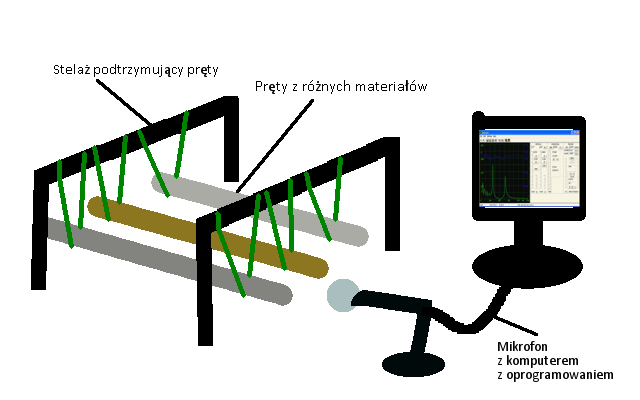
\includegraphics[scale=0.5]{schemat}
		\caption{Schemat układu pomiarowego}
		\label{schematUkladu}
	\end{figure}
	
%--------------------------------------------------------------------------------------------------------------
	
	\section{Wykonanie ćwiczenia}
	Wykonanie ćwiczenia dzieli się na dwa kroki stosowane dla każdego badanego pręta oraz jednej wspólnej analizy wyników.
	\subsection{Pomiary specyfikacji prętów}
	\begin{itemize}
		\item Pomiar długości pręta za pomocą miary zwijanej.
		\item Pomiar grubości pręta za pomocą suwmiarki (w przypadku otwartego walca mierzymy promień zewnętrzny i wewnętrzny).
		\item Zważenie pręta w najlepszy możliwy sposób za pomocą wagi elektronicznej.
		\item Zapisanie wyników o danym ciele do tabeli.
	\end{itemize}

	\subsection{Pomiar częstotliwości harmonicznych}
	\begin{itemize}
		\item Osadzenie preta w niciach zamontowanych do stelaża.
		\item Przybliżenie mikrofonu do badanego pręta.
		\item Uderzenie młotkiem w pręt aby wprawić go w drganie.
		\item Zamrożenie odczytu programu Zelscope w momencie najlepszej widoczności widma fal harmonicznych.
		\item Odczyt sześciu pierwszych harmonicznych (jeżeli taką ilość udało się zaobserwować).
	\end{itemize}
	W przypadku niejednoznacznego odczytu częstotliwości harmonicznych nalezy powtórzyć pomiar.
	
	\subsection{Oblicznanie koniecznych wartości}
	Z zapisanych danych pomiarowych należy obliczyć gęstość ciała daną wzorem:
	\begin{equation}
		\rho = \frac{m}{V}
	\end{equation}
	gdzie $m$ to zmierzona masa ciała oraz $V$ to objętość ciała obliczona odpowiednio dla każdego pręta z odpowiednich wielkości. Pręty są różnymi figurami przestrzennymi, przez wykorzystujemy odpowiedni wzór dla:
	\begin{itemize}
		\item walca o promieniu podstawy $r$ oraz wysokości $h$
		\begin{equation}
			V = \pi r^2 h
		\end{equation}
		
		\item prostopadłościanu prawidłowego czworokątnego o krawędzi podstawy $a$ oraz wysokości $h$
		\begin{equation}
			V = a^2 h
		\end{equation}
		
		\item otwartego walca o promieniu zewnętrznym podstawy $R$, promieniu wewnętrznym podstawy $r$ oraz wysokości $h$
		\begin{equation}
			V = \pi (R^2 - r^2) h
		\end{equation}
	\end{itemize}
	Do oblicznia długości fali $\lambda$ zastosujemy zależność od częstotliwości:
	\begin{equation}
		\lambda = \frac{1}{f}
	\end{equation}
	Odległość $l$ między węzłami fali stojącej stanowi połowę jej długości:
	\begin{equation}
		l = \frac{1}{2} \lambda
	\end{equation}
	Do obliczenia predkości rozchodzenia się fali zastosujemy wzór:
	\begin{equation}
		V = 2lf
	\end{equation}
		
%--------------------------------------------------------------------------------------------------------------
	
	\section{Opracowanie danych pomiarowych}
	
	%----------------------------------------------------------------------------------------------------------	
	
	\subsection{Analiza niepewności}
	
%--------------------------------------------------------------------------------------------------------------

	\section{Podsumowanie}

%--------------------------------------------------------------------------------------------------------------

	\section{Wnioski}
	
\end{document}